% bare_conf.tex
%% V1.3
%% 2007/01/11
%% by Michael Shell
%% See:
%% http://www.michaelshell.org/
%% for current contact information.
%%
%% This is a skeleton file demonstrating the use of IEEEtran.cls
%% (requires IEEEtran.cls version 1.7 or later) with an IEEE conference paper.
%%
%% Support sites:
%% http://www.michaelshell.org/tex/ieeetran/
%% http://www.ctan.org/tex-archive/macros/latex/contrib/IEEEtran/
%% and
%% http://www.ieee.org/

%%*************************************************************************
%% Legal Notice:
%% This code is offered as-is without any warranty either expressed or
%% implied; without even the implied warranty of MERCHANTABILITY or
%% FITNESS FOR A PARTICULAR PURPOSE! 
%% User assumes all risk.
%% In no event shall IEEE or any contributor to this code be liable for
%% any damages or losses, including, but not limited to, incidental,
%% consequential, or any other damages, resulting from the use or misuse
%% of any information contained here.
%%
%% All comments are the opinions of their respective authors and are not
%% necessarily endorsed by the IEEE.
%%
%% This work is distributed under the LaTeX Project Public License (LPPL)
%% ( http://www.latex-project.org/ ) version 1.3, and may be freely used,
%% distributed and modified. A copy of the LPPL, version 1.3, is included
%% in the base LaTeX documentation of all distributions of LaTeX released
%% 2003/12/01 or later.
%% Retain all contribution notices and credits.
%% ** Modified files should be clearly indicated as such, including  **
%% ** renaming them and changing author support contact information. **
%%
%% File list of work: IEEEtran.cls, IEEEtran_HOWTO.pdf, bare_adv.tex,
%%                    bare_conf.tex, bare_jrnl.tex, bare_jrnl_compsoc.tex
%%*************************************************************************

% *** Authors should verify (and, if needed, correct) their LaTeX system  ***
% *** with the testflow diagnostic prior to trusting their LaTeX platform ***
% *** with production work. IEEE's font choices can trigger bugs that do  ***
% *** not appear when using other class files.                            ***
% The testflow support page is at:
% http://www.michaelshell.org/tex/testflow/



% Note that the a4paper option is mainly intended so that authors in
% countries using A4 can easily print to A4 and see how their papers will
% look in print - the typesetting of the document will not typically be
% affected with changes in paper size (but the bottom and side margins will).
% Use the testflow package mentioned above to verify correct handling of
% both paper sizes by the user's LaTeX system.
%
% Also note that the "draftcls" or "draftclsnofoot", not "draft", option
% should be used if it is desired that the figures are to be displayed in
% draft mode.
%
\documentclass[conference]{IEEEtran}
% Add the compsoc option for Computer Society conferences.
%
% If IEEEtran.cls has not been installed into the LaTeX system files,
% manually specify the path to it like:
% \documentclass[conference]{../sty/IEEEtran}

\usepackage{balance}



% Some very useful LaTeX packages include:
% (uncomment the ones you want to load)


% *** MISC UTILITY PACKAGES ***
%
%\usepackage{ifpdf}
% Heiko Oberdiek's ifpdf.sty is very useful if you need conditional
% compilation based on whether the output is pdf or dvi.
% usage:
% \ifpdf
%   % pdf code
% \else
%   % dvi code
% \fi
% The latest version of ifpdf.sty can be obtained from:
% http://www.ctan.org/tex-archive/macros/latex/contrib/oberdiek/
% Also, note that IEEEtran.cls V1.7 and later provides a builtin
% \ifCLASSINFOpdf conditional that works the same way.
% When switching from latex to pdflatex and vice-versa, the compiler may
% have to be run twice to clear warning/error messages.






% *** CITATION PACKAGES ***
%
\usepackage{cite}
% cite.sty was written by Donald Arseneau
% V1.6 and later of IEEEtran pre-defines the format of the cite.sty package
% \cite{} output to follow that of IEEE. Loading the cite package will
% result in citation numbers being automatically sorted and properly
% "compressed/ranged". e.g., [1], [9], [2], [7], [5], [6] without using
% cite.sty will become [1], [2], [5]--[7], [9] using cite.sty. cite.sty's
% \cite will automatically add leading space, if needed. Use cite.sty's
% noadjust option (cite.sty V3.8 and later) if you want to turn this off.
% cite.sty is already installed on most LaTeX systems. Be sure and use
% version 4.0 (2003-05-27) and later if using hyperref.sty. cite.sty does
% not currently provide for hyperlinked citations.
% The latest version can be obtained at:
% http://www.ctan.org/tex-archive/macros/latex/contrib/cite/
% The documentation is contained in the cite.sty file itself.


% Meto paquetes a huevo
\usepackage{graphicx}
\usepackage[table]{xcolor}

% *** GRAPHICS RELATED PACKAGES ***
%
%\ifCLASSINFOpdf
  % \usepackage[pdftex]{graphicx}
  % declare the path(s) where your graphic files are
  % \graphicspath{{../pdf/}{../jpeg/}}
  % and their extensions so you won't have to specify these with
  % every instance of \includegraphics
  % \DeclareGraphicsExtensions{.pdf,.jpeg,.png}
%\else
  % or other class option (dvipsone, dvipdf, if not using dvips). graphicx
  % will default to the driver specified in the system graphics.cfg if no
  % driver is specified.
  % \usepackage[dvips]{graphicx}
  % declare the path(s) where your graphic files are
  % \graphicspath{{../eps/}}
  % and their extensions so you won't have to specify these with
  % every instance of \includegraphics
  % \DeclareGraphicsExtensions{.eps}
%\fi
% graphicx was written by David Carlisle and Sebastian Rahtz. It is
% required if you want graphics, photos, etc. graphicx.sty is already
% installed on most LaTeX systems. The latest version and documentation can
% be obtained at: 
% http://www.ctan.org/tex-archive/macros/latex/required/graphics/
% Another good source of documentation is "Using Imported Graphics in
% LaTeX2e" by Keith Reckdahl which can be found as epslatex.ps or
% epslatex.pdf at: http://www.ctan.org/tex-archive/info/
%
% latex, and pdflatex in dvi mode, support graphics in encapsulated
% postscript (.eps) format. pdflatex in pdf mode supports graphics
% in .pdf, .jpeg, .png and .mps (metapost) formats. Users should ensure
% that all non-photo figures use a vector format (.eps, .pdf, .mps) and
% not a bitmapped formats (.jpeg, .png). IEEE frowns on bitmapped formats
% which can result in "jaggedy"/blurry rendering of lines and letters as
% well as large increases in file sizes.
%
% You can find documentation about the pdfTeX application at:
% http://www.tug.org/applications/pdftex





% *** MATH PACKAGES ***
%
\usepackage[cmex10]{amsmath}
% A popular package from the American Mathematical Society that provides
% many useful and powerful commands for dealing with mathematics. If using
% it, be sure to load this package with the cmex10 option to ensure that
% only type 1 fonts will utilized at all point sizes. Without this option,
% it is possible that some math symbols, particularly those within
% footnotes, will be rendered in bitmap form which will result in a
% document that can not be IEEE Xplore compliant!
%
% Also, note that the amsmath package sets \interdisplaylinepenalty to 10000
% thus preventing page breaks from occurring within multiline equations. Use:
%\interdisplaylinepenalty=2500
% after loading amsmath to restore such page breaks as IEEEtran.cls normally
% does. amsmath.sty is already installed on most LaTeX systems. The latest
% version and documentation can be obtained at:
% http://www.ctan.org/tex-archive/macros/latex/required/amslatex/math/





% *** SPECIALIZED LIST PACKAGES ***
%
%\usepackage{algorithmic}
% algorithmic.sty was written by Peter Williams and Rogerio Brito.
% This package provides an algorithmic environment fo describing algorithms.
% You can use the algorithmic environment in-text or within a figure
% environment to provide for a floating algorithm. Do NOT use the algorithm
% floating environment provided by algorithm.sty (by the same authors) or
% algorithm2e.sty (by Christophe Fiorio) as IEEE does not use dedicated
% algorithm float types and packages that provide these will not provide
% correct IEEE style captions. The latest version and documentation of
% algorithmic.sty can be obtained at:
% http://www.ctan.org/tex-archive/macros/latex/contrib/algorithms/
% There is also a support site at:
% http://algorithms.berlios.de/index.html
% Also of interest may be the (relatively newer and more customizable)
% algorithmicx.sty package by Szasz Janos:
% http://www.ctan.org/tex-archive/macros/latex/contrib/algorithmicx/




% *** ALIGNMENT PACKAGES ***
%
%\usepackage{array}
% Frank Mittelbach's and David Carlisle's array.sty patches and improves
% the standard LaTeX2e array and tabular environments to provide better
% appearance and additional user controls. As the default LaTeX2e table
% generation code is lacking to the point of almost being broken with
% respect to the quality of the end results, all users are strongly
% advised to use an enhanced (at the very least that provided by array.sty)
% set of table tools. array.sty is already installed on most systems. The
% latest version and documentation can be obtained at:
% http://www.ctan.org/tex-archive/macros/latex/required/tools/


%\usepackage{mdwmath}
%\usepackage{mdwtab}
% Also highly recommended is Mark Wooding's extremely powerful MDW tools,
% especially mdwmath.sty and mdwtab.sty which are used to format equations
% and tables, respectively. The MDWtools set is already installed on most
% LaTeX systems. The lastest version and documentation is available at:
% http://www.ctan.org/tex-archive/macros/latex/contrib/mdwtools/


% IEEEtran contains the IEEEeqnarray family of commands that can be used to
% generate multiline equations as well as matrices, tables, etc., of high
% quality.


%\usepackage{eqparbox}
% Also of notable interest is Scott Pakin's eqparbox package for creating
% (automatically sized) equal width boxes - aka "natural width parboxes".
% Available at:
% http://www.ctan.org/tex-archive/macros/latex/contrib/eqparbox/





% *** SUBFIGURE PACKAGES ***
%\usepackage[tight,footnotesize]{subfigure}
% subfigure.sty was written by Steven Douglas Cochran. This package makes it
% easy to put subfigures in your figures. e.g., "Figure 1a and 1b". For IEEE
% work, it is a good idea to load it with the tight package option to reduce
% the amount of white space around the subfigures. subfigure.sty is already
% installed on most LaTeX systems. The latest version and documentation can
% be obtained at:
% http://www.ctan.org/tex-archive/obsolete/macros/latex/contrib/subfigure/
% subfigure.sty has been superceeded by subfig.sty.



%\usepackage[caption=false]{caption}
%\usepackage[font=footnotesize]{subfig}
% subfig.sty, also written by Steven Douglas Cochran, is the modern
% replacement for subfigure.sty. However, subfig.sty requires and
% automatically loads Axel Sommerfeldt's caption.sty which will override
% IEEEtran.cls handling of captions and this will result in nonIEEE style
% figure/table captions. To prevent this problem, be sure and preload
% caption.sty with its "caption=false" package option. This is will preserve
% IEEEtran.cls handing of captions. Version 1.3 (2005/06/28) and later 
% (recommended due to many improvements over 1.2) of subfig.sty supports
% the caption=false option directly:
%\usepackage[caption=false,font=footnotesize]{subfig}
%
% The latest version and documentation can be obtained at:
% http://www.ctan.org/tex-archive/macros/latex/contrib/subfig/
% The latest version and documentation of caption.sty can be obtained at:
% http://www.ctan.org/tex-archive/macros/latex/contrib/caption/




% *** FLOAT PACKAGES ***
%
%\usepackage{fixltx2e}
% fixltx2e, the successor to the earlier fix2col.sty, was written by
% Frank Mittelbach and David Carlisle. This package corrects a few problems
% in the LaTeX2e kernel, the most notable of which is that in current
% LaTeX2e releases, the ordering of single and double column floats is not
% guaranteed to be preserved. Thus, an unpatched LaTeX2e can allow a
% single column figure to be placed prior to an earlier double column
% figure. The latest version and documentation can be found at:
% http://www.ctan.org/tex-archive/macros/latex/base/


\usepackage{subfig}
%\usepackage{stfloats}
% stfloats.sty was written by Sigitas Tolusis. This package gives LaTeX2e
% the ability to do double column floats at the bottom of the page as well
% as the top. (e.g., "\begin{figure*}[!b]" is not normally possible in
% LaTeX2e). It also provides a command:
%\fnbelowfloat
% to enable the placement of footnotes below bottom floats (the standard
% LaTeX2e kernel puts them above bottom floats). This is an invasive package
% which rewrites many portions of the LaTeX2e float routines. It may not work
% with other packages that modify the LaTeX2e float routines. The latest
% version and documentation can be obtained at:
% http://www.ctan.org/tex-archive/macros/latex/contrib/sttools/
% Documentation is contained in the stfloats.sty comments as well as in the
% presfull.pdf file. Do not use the stfloats baselinefloat ability as IEEE
% does not allow \baselineskip to stretch. Authors submitting work to the
% IEEE should note that IEEE rarely uses double column equations and
% that authors should try to avoid such use. Do not be tempted to use the
% cuted.sty or midfloat.sty packages (also by Sigitas Tolusis) as IEEE does
% not format its papers in such ways.





% *** PDF, URL AND HYPERLINK PACKAGES ***
%
\usepackage{url}
% url.sty was written by Donald Arseneau. It provides better support for
% handling and breaking URLs. url.sty is already installed on most LaTeX
% systems. The latest version can be obtained at:
% http://www.ctan.org/tex-archive/macros/latex/contrib/misc/
% Read the url.sty source comments for usage information. Basically,
% \url{my_url_here}.





% *** Do not adjust lengths that control margins, column widths, etc. ***
% *** Do not use packages that alter fonts (such as pslatex).         ***
% There should be no need to do such things with IEEEtran.cls V1.6 and later.
% (Unless specifically asked to do so by the journal or conference you plan
% to submit to, of course. )


% correct bad hyphenation here
\hyphenation{op-tical net-works semi-conduc-tor}

% lindo
\newcommand{\refp}[1]{(\ref{#1})}

\begin{document}
%
% paper title
% can use linebreaks \\ within to get better formatting as desired
\title{\Huge \bf \sc
Calibration of an inertial measurement unit}


% author names and affiliations
% use a multiple column layout for up to three different
% affiliations
\author{\IEEEauthorblockN{Santiago Paternain}
\IEEEauthorblockA{Facultad de Ingeniería\\
Universidad de la República\\
Montevideo, Uruguay\\
spaternain@gmail.com}
\and
\IEEEauthorblockN{Mat\'ias Tailani\'an}
\IEEEauthorblockA{Facultad de Ingeniería\\
Universidad de la República\\
Montevideo, Uruguay\\
matias@tailanian.com}
\and
\IEEEauthorblockN{Rafael Canetti}
\IEEEauthorblockA{Facultad de Ingeniería\\
Universidad de la República\\
Montevideo, Uruguay\\
canetti@fing.edu.uy}
}

% conference papers do not typically use \thanks and this command
% is locked out in conference mode. If really needed, such as for
% the acknowledgment of grants, issue a \IEEEoverridecommandlockouts
% after \documentclass

% for over three affiliations, or if they all won't fit within the width
% of the page, use this alternative format:
% 
%\author{\IEEEauthorblockN{Michael Shell\IEEEauthorrefmark{1},
%Homer Simpson\IEEEauthorrefmark{2},
%James Kirk\IEEEauthorrefmark{3}, 
%Montgomery Scott\IEEEauthorrefmark{3} and
%Eldon Tyrell\IEEEauthorrefmark{4}}
%\IEEEauthorblockA{\IEEEauthorrefmark{1}School of Electrical and Computer Engineering\\
%Georgia Institute of Technology,
%Atlanta, Georgia 30332--0250\\ Email: see http://www.michaelshell.org/contact.html}
%\IEEEauthorblockA{\IEEEauthorrefmark{2}Twentieth Century Fox, Springfield, USA\\
%Email: homer@thesimpsons.com}
%\IEEEauthorblockA{\IEEEauthorrefmark{3}Starfleet Academy, San Francisco, California 96678-2391\\
%Telephone: (800) 555--1212, Fax: (888) 555--1212}
%\IEEEauthorblockA{\IEEEauthorrefmark{4}Tyrell Inc., 123 Replicant Street, Los Angeles, California 90210--4321}}




% use for special paper notices
%\IEEEspecialpapernotice{(Invited Paper)}




% make the title area
\maketitle


\begin{abstract}
%\boldmath
This paper presents a fast and low cost way to calibrate different inertial measurement sensors. In particular we present the calibration of an accelerometer and a gyroscope using nonlinear least squares. A model of the sensors is presented based on the main errors that MEMS devices present, a calibration method is proposed for the static parameters of the model. Finally a temperature adjust is made.  
% -cambio-
\end{abstract}
% IEEEtran.cls defaults to using nonbold math in the Abstract.
% This preserves the distinction between vectors and scalars. However,
% if the conference you are submitting to favors bold math in the abstract,
% then you can use LaTeX's standard command \boldmath at the very start
% of the abstract to achieve this. Many IEEE journals/conferences frown on
% math in the abstract anyway.

% no keywords




% For peer review papers, you can put extra information on the cover
% page as needed:
% \ifCLASSOPTIONpeerreview
% \begin{center} \bfseries EDICS Category: 3-BBND \end{center}
% \fi
%
% For peerreview papers, this IEEEtran command inserts a page break and
% creates the second title. It will be ignored for other modes.
\IEEEpeerreviewmaketitle

\section{Introduction}
The development of the Micro-electromechanical Systems (MEMS) technology has allowed to manufacture many low-cost chip-sensors, such as accelerometers, gyroscopes and magnetometers. Those chips have been adopted in many applications, for instance Inertial Navigation Systems  (INS)\cite{bib:un_puto_nuevo}. However this sensors have many error sources, thus they must be calibrated before being used and they should be re-calibrated periodically for any precision application. The different sources of error will be analysed in more detail in section \refp{sec:modelo} and the implications of those errors will be derived.\\ 

The calibration proposed in this work is tested on a 3-axis accelerometer \emph{ADXL345} of \emph{Analog Devices} and a 3-axis gyroscope \emph{ITG-3200} of \emph{InvenSense}, yet the model developed and the methodology can be used in other devices because the model is based on common characteristics of MEMS sensors. The sensors named before are included in a Inertial Measurement Unit(IMU): The Mongoose (figure \refp{fig:mongoose}). \\

The motivation for this calibration is to have enough precision to estimate the state of an Unmanned Aerial Vehicle (UAV) with quadrotor architecture.\\

The first step of the calibration is to obtain the static parameters of the devices for the ambiance temperature. This step is based on knowing the exact orientation of the IMU for the calibration of both sensors and the exact angular speed for the gyroscope calibration. Other related works waive this requirement\cite{bib:calib_imu, bib:kalman} and uses the fact that in any position angular speed (for the gyroscope calibration) and gravity vector (for the accelerometer calibration) are constant.\\

\begin{figure}[h]
	\centering
	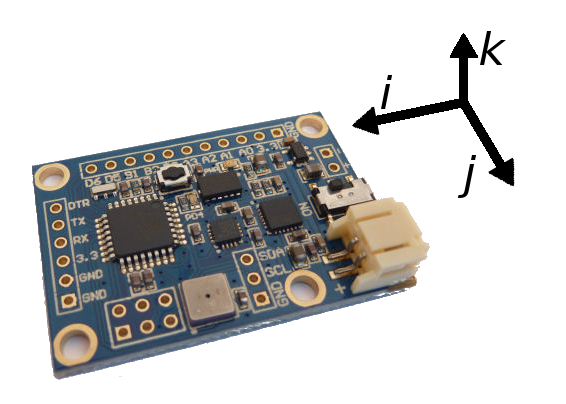
\includegraphics[width=.6\columnwidth]{./pics_paper/mongoose.png}
	\caption{\textbf{Mongoose -} Inertial Measurement Unit used. Red arrows represent the axis platform $S - \{\hat{i}, \hat{j}, \hat{k} \}$. }
	\label{fig:mongoose}
\end{figure}

We take in consideration a fact that is not usually taken into account in the literature (see \cite{bib:calib_imu}, \cite{bib:kalman}, \cite{bib:calib_imu_dos}): the measures given by this sensors are not independent of the temperature. Many devices that uses MEMS sensors need to work properly in a wide temperature range. In other cases, the temperature in operation of the system is different(for instance due to Joule Effect of the wires near the sensors) than the ambiance temperature in which the sensor was calibrated. Therefore a temperature adjust must be made.
   
\section{Model of the sensors}
\label{sec:modelo}

As it was stated before, there exist many error sources in MEMS devices. In \cite{bib:calib_imu} two of this sources are mentioned: the nonlinear response of the sensors and the non-orthogonality of the axis of the sensor. In addition we can observe also that it exist an electric noise in the measures (Figure \ref{fig:noise}) and a dependence of the temperature.\\
\vspace{-10pt}
\begin{figure}[h!]
  \centering
  \subfloat[Accelerometer data $\hat{k}$]{\label{fig:angulos_1}
  		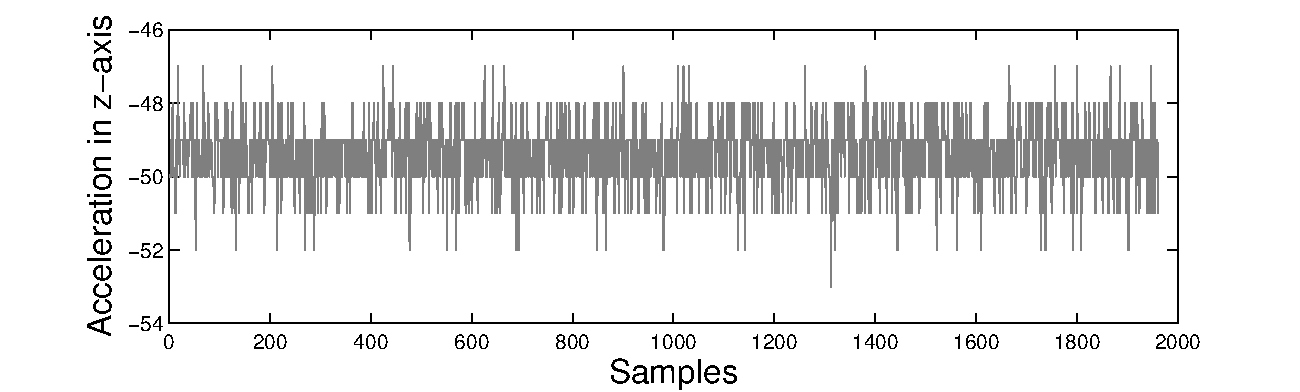
\includegraphics[width=1\columnwidth]
  			{./pics_paper/acc_noise.pdf}}\\[-5pt]
  			\vspace{-5pt}
  \subfloat[Gyroscope data $\hat{j}$]{\label{fig:angulos_2} 
  		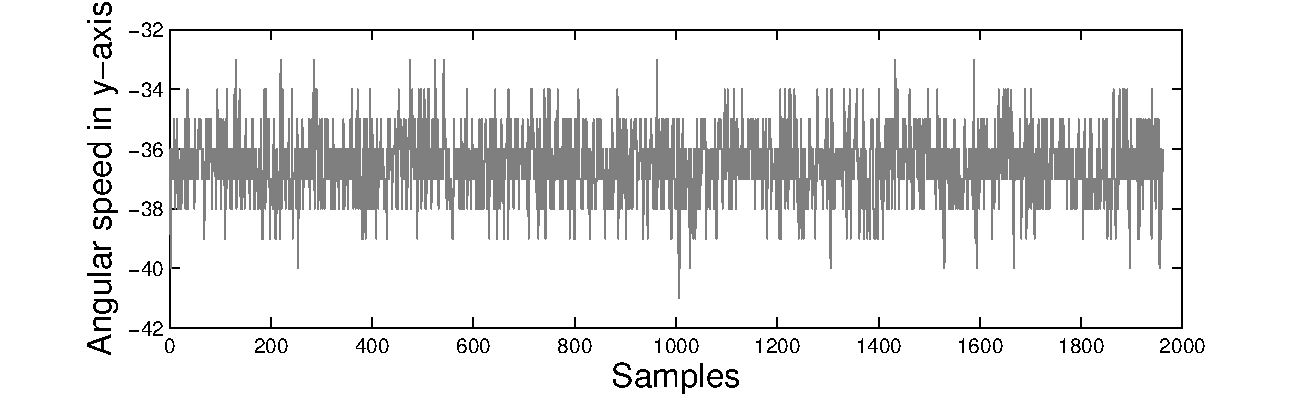
\includegraphics[width=1\columnwidth]
  			{./pics_paper/gyro_noise.pdf}}
  \caption{\textbf{Noise -} Measures from accelerometer and gyroscope in static equilibrium.}
  \label{fig:noise}
\end{figure}

According to the datasheets of the devices (\cite{bib:acc_data, bib:gyro_data}), effect of nonlinearities represent the $\pm 0.5.\%$  of the full scale for the accelerometer and the $\pm 0.2\%$ for the gyroscope. Therefore, this effect is not considered and after the calibration, it must be verified.\\
%TODO Al final hacer las cuentas para ver que es despreciable.

In Figure \refp{fig:noise} we can observe that the electrical noise of the devices is typically 3 LSB (Least Significant Bit) peak to peak, which (according to the datasheets \cite{bib:acc_data, bib:gyro_data}) correspond to $11.7 mg$ and $0.21 ^{\circ}/s $. The error is not biased, thus, we not need to consider it, because many samples are used in the procedure and the effect vanishes.\\

Based on the assumption that both sensors have a linear response and considering the non-orthogonality of the axis of the devices we are going to present a standard model for both sensors (see \cite{bib:calib_imu}, \cite{bib:kalman}, \cite{bib:calib_imu_dos}).

\subsection{Accelerometer}
Due to construction issues the sensitivity axis of the device are generally not orthogonal. Lets define a platform system as shown in Figure \refp{fig:mongoose}. Let $\mathbf{a}^a$ be the true acceleration (meaning the theoretical acceleration measured in $ms^{-2}$) expressed in the sensitivity axis of the accelerometer and let $\mathbf{a}^p$ be the theoretical true acceleration (also measured in $ms^{-2}$) expressed in the platform system. The two acceleration vectors are related according to equation \refp{eq:nonorto}:
\begin{equation}
\mathbf{a}^p = \mathbf{T}_a^p\mathbf{a}^a, \; \mathbf{T}_a^p = \left(\begin{array}{ccc}
1 & - \alpha_{yz} & \alpha_{zy}\\
\alpha_{xz} & 1 & - \alpha_{zx}\\
-\alpha_{xy} & \alpha_{yx} & 1
\end{array}\right)
\label{eq:nonorto}
\end{equation}
In equation \refp{eq:nonorto}, scalars $\alpha_{ij}$ represents the rotation of the $i-th$ sensitivity axis of the accelerometer over the $j-th$ axis of the platform system. In Figure \refp{fig:nonorto} this relation can be observed graphically. Since those errors are due to the manufacturing process we will assume that they will remain constant long enough.

\begin{figure}
	\centering
	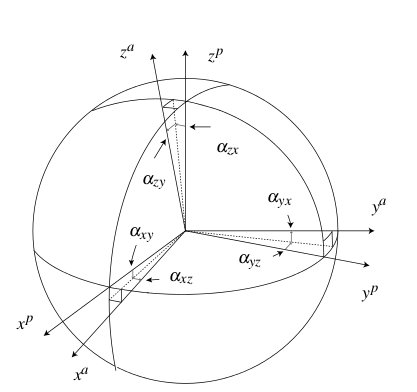
\includegraphics[width=.6\columnwidth]{./pics_paper/ejes_acc.jpg}
	\caption{\textbf{Non orthogonality -} Rotations of the sensitivity axis of the accelerometer over the axis of the platform system.}
	\label{fig:nonorto}
\end{figure}

As it was stated before, a linear model between the acceleration measured in the sensitivity axis and the true acceleration in the same system is considered. Thus we have:
\begin{equation}
\tilde{\mathbf{a}}^a = \mathbf{K}_a\mathbf{a}^a + \mathbf{b}_a
\label{eq:modlineal}
\end{equation}
In equation \refp{eq:modlineal}, $\tilde{\mathbf{a}}^a$ is the measure obtained by the accelerometer (measured in bits), $\mathbf{K}_a$ is a diagonal matrix that represents the sensitivity of each axis and $\mathbf{b}_a$ is a vector that represent the bias of each axis. Those parameters may variate as the temperature changes. However, constant temperature is considered. Using equations \refp{eq:nonorto} and \refp{eq:modlineal} we can establish a model of the accelerometer:

\begin{equation}
\tilde{\mathbf{a}}^a = \mathbf{K}_a\mathbf{T}_p^a\mathbf{a}^p + \mathbf{b}_a = \mathbf{K}_a(\mathbf{T}_a^p)^{-1}\mathbf{a}^p + \mathbf{b}_a 
\end{equation}


\subsection{Gyroscope}
The error sources consider in the case of the gyroscope are the same that we developed for the accelerometer. Thus, we are going to consider the same model:

\begin{equation}
\tilde{\boldsymbol{\omega}}_a = \mathbf{K}_{\omega}(\mathbf{T}_{\omega}^p)^{-1}\boldsymbol{\omega}^p+\mathbf{b}_{\omega}
\end{equation}

\section{Calibration method proposed}
The problem of calibration is to establish the values for the unknown parameters of the model that adjust ``the better'' a certain set of data. This criterion will be defined in Section \refp{sec:param}. 


\subsection{Static Parameter Calibration}
\label{sec:param}

Let $\boldsymbol{\theta}_s$ (where the subindex $s$ refers to a sensor) be the parameter vector of a certain sensor. We can define this vector as:
\begin{equation}
\boldsymbol{\theta} = [k_{sx},k_{sy},k_{sy},b_{sx},b_{sy},b_{sy}, \alpha_{sxy},\alpha_{sxz},\alpha_{syx},\alpha_{syz},\alpha_{szx},\alpha_{szy}]^T
\label{eq:theta}
\end{equation}

In equation \refp{eq:theta}, $k_{si}$, with $i=1,2,3$ are the diagonal elements of the matrix $\mathbf{K}_s$, $b_{si}$, with $i = 1,2,3$ are the elements of vector $\mathbf{b}_s$ and $\alpha_{sij}$, with $i = 1,2,3$, $j = 1,2,3$ and $i \neq j$ are the elements outside the diagonal of the matrix $\mathbf{T}_s^p$.\\

As adjust criterion we choose to minimize the sum of the squares of the norms of the differences between true acceleration and measured acceleration. This problem can be written as follows:

\begin{equation}
\min_{\boldsymbol{\theta}} \sum_{i = 1}^M ||\mathbf{s}_i^p - \mathbf{T}_s^p(\mathbf{K_s})^{-1}(\tilde{\mathbf{s}}_i^s-\mathbf{b}_s) ||^2
\label{eq:calib_problem}
\end{equation}

In equation \refp{eq:calib_problem}, $M$ is the cardinal of the training set, $\mathbf{s}_i^p$ is the true magnitude (acceleration or angular speed) and $\tilde{\mathbf{s}}_i$ are the values given by the sensor.\\

It is important to consider that the minimize function will generally have more than one local minimum. To ensure that the solution obtained is the desired one, the seed for the algorithm must be carefully chosen. Thus, datasheet values of the parameters are chosen as seed for the optimization.

Typically we will choose a vector $\boldsymbol{\theta}_0$ that is close to the values of the unknown parameters. Even if we do not know the exact value of the model's parameters, the datasheet of the different sensors can give us a very good clue about those values.\\

\subsubsection{Accelerometer}
\label{subsec:acc}
Since an accelerometer measures the acceleration in a free fall referential, in static equilibrium it will measure an acceleration that has as norm the gravitational constant of the  earth ($g = 9.81ms^{-2}$), its direction is collinear with the line defined by the position of the accelerometer and the center of the earth and its sense is from the center of the earth towards the position of the accelerometer, meaning ``up''. This allows to have an exact expression for the acceleration, the procedure used consist in measureing magnitude with different orientations of the acceleration and then solve the problem stated in equation \refp{eq:calib_problem}.\\

The 27 measures made were the following:
\begin{itemize}
\item Starting position: $x$ axis pointing ``down'': 9 measures were made combining two rotations. First, rotating around the $z$ axis $\theta =0^\circ, 10^\circ, 20^\circ, 30^\circ, 45^\circ$. Then, for each angle defined(except for $\theta = 0^\circ$), two measures were made rotating around the $x$ axis $\psi = 0^\circ, -45^\circ$. This set of measures can be expressed in the following way:
\begin{scriptsize}
\begin{equation}
\mathbf{a}^p = \left(\begin{array}{ccc}
1 & 0 & 0\\
0 & \cos \psi & \sin \psi \\
0 & -\sin \psi & \cos \psi
\end{array}\right)\left(\begin{array}{ccc}
\cos \theta & \sin \theta & 0\\
-\sin \theta & \cos \theta & 0\\
0 & 0 & 1
\end{array}\right)\left(\begin{array}{c}
-g\\
0\\
0
\end{array}\right)
\label{eq:acc_x}
\end{equation}
\end{scriptsize}
 

\item Starting position: $y$ axis pointing ``up'': 9 measures were made combining two rotations. First, rotating around the $x$ axis $\psi =0^\circ, 10^\circ, 20^\circ, 30^\circ, 45^\circ$. Then, for each angle defined(except for $\theta = 0^\circ$), two measures were made rotating around the $y$ axis $\varphi = 0^\circ, 45^\circ$.   

\begin{scriptsize}
\begin{equation}
\mathbf{a}^p = \left(\begin{array}{ccc}
\cos \varphi & 0 &\sin \varphi\\
0 & 1 & 0\\
-\sin \varphi & 0 & \cos \varphi
\end{array}\right)\left(\begin{array}{ccc}
1 & 0 & 0\\
0 & \cos \psi & \sin \psi \\
0 & -\sin \psi & \cos \psi
\end{array}\right)\left(\begin{array}{c}
0\\
g\\
0
\end{array}\right)
\label{eq:acc_y}
\end{equation}
\end{scriptsize}

\item Starting position: $z$ axis pointing ``up'': 9 measures were made combining two rotations. First, rotating around the $y$ axis: $\phi =0^\circ, -10^\circ, -20^\circ, -30^\circ, -45^\circ$. Then, for each angle defined(except for $\phi = 0^\circ$), two measures were made rotating around the $z$ axis $\theta = 0^\circ, 45^\circ$.   \end{itemize}

\begin{scriptsize}
\begin{equation}
\mathbf{a}^p = \left(\begin{array}{ccc}
\cos \theta & \sin \theta & 0\\
-\sin \theta & \cos \theta & 0\\
0 & 0 & 1
\end{array}\right)\left(\begin{array}{ccc}
\cos \varphi & 0 &\sin \varphi\\
0 & 1 & 0\\
-\sin \varphi & 0 & \cos \varphi
\end{array}\right)\left(\begin{array}{c}
0\\
0\\
g
\end{array}\right)
\label{eq:acc_z}
\end{equation}
\end{scriptsize}

The 27 measures are separated in two sets: 14 used for optimization and 13 as test set.\\

The key issue is knowing the orientation of the platform. Having solved this, it is easy to compute the theoretical acceleration that the device should measure in each axis from equations \refp{eq:acc_x}, \refp{eq:acc_y} and \refp{eq:acc_z}.\\

First of all, we attached the platform to a wooden cube. This allows us to perform $90^\circ$ rotations, thus if we had an horizontal surface we can take measures with the gravity vector aligned to any of three axis. The horizontal surface was assured using a three leg adjustable table (see Figure \refp{fig:mesa}). In addition this table allows us to perform rotations of known angles using a scaled semicircle and a pendulum as it is shown also in Figure \refp{fig:mesa}. The rotations over the second axis were made using a carpenter's square, therefore we have a proper $45^\circ$ rotation.\\

\begin{figure}
	\centering
	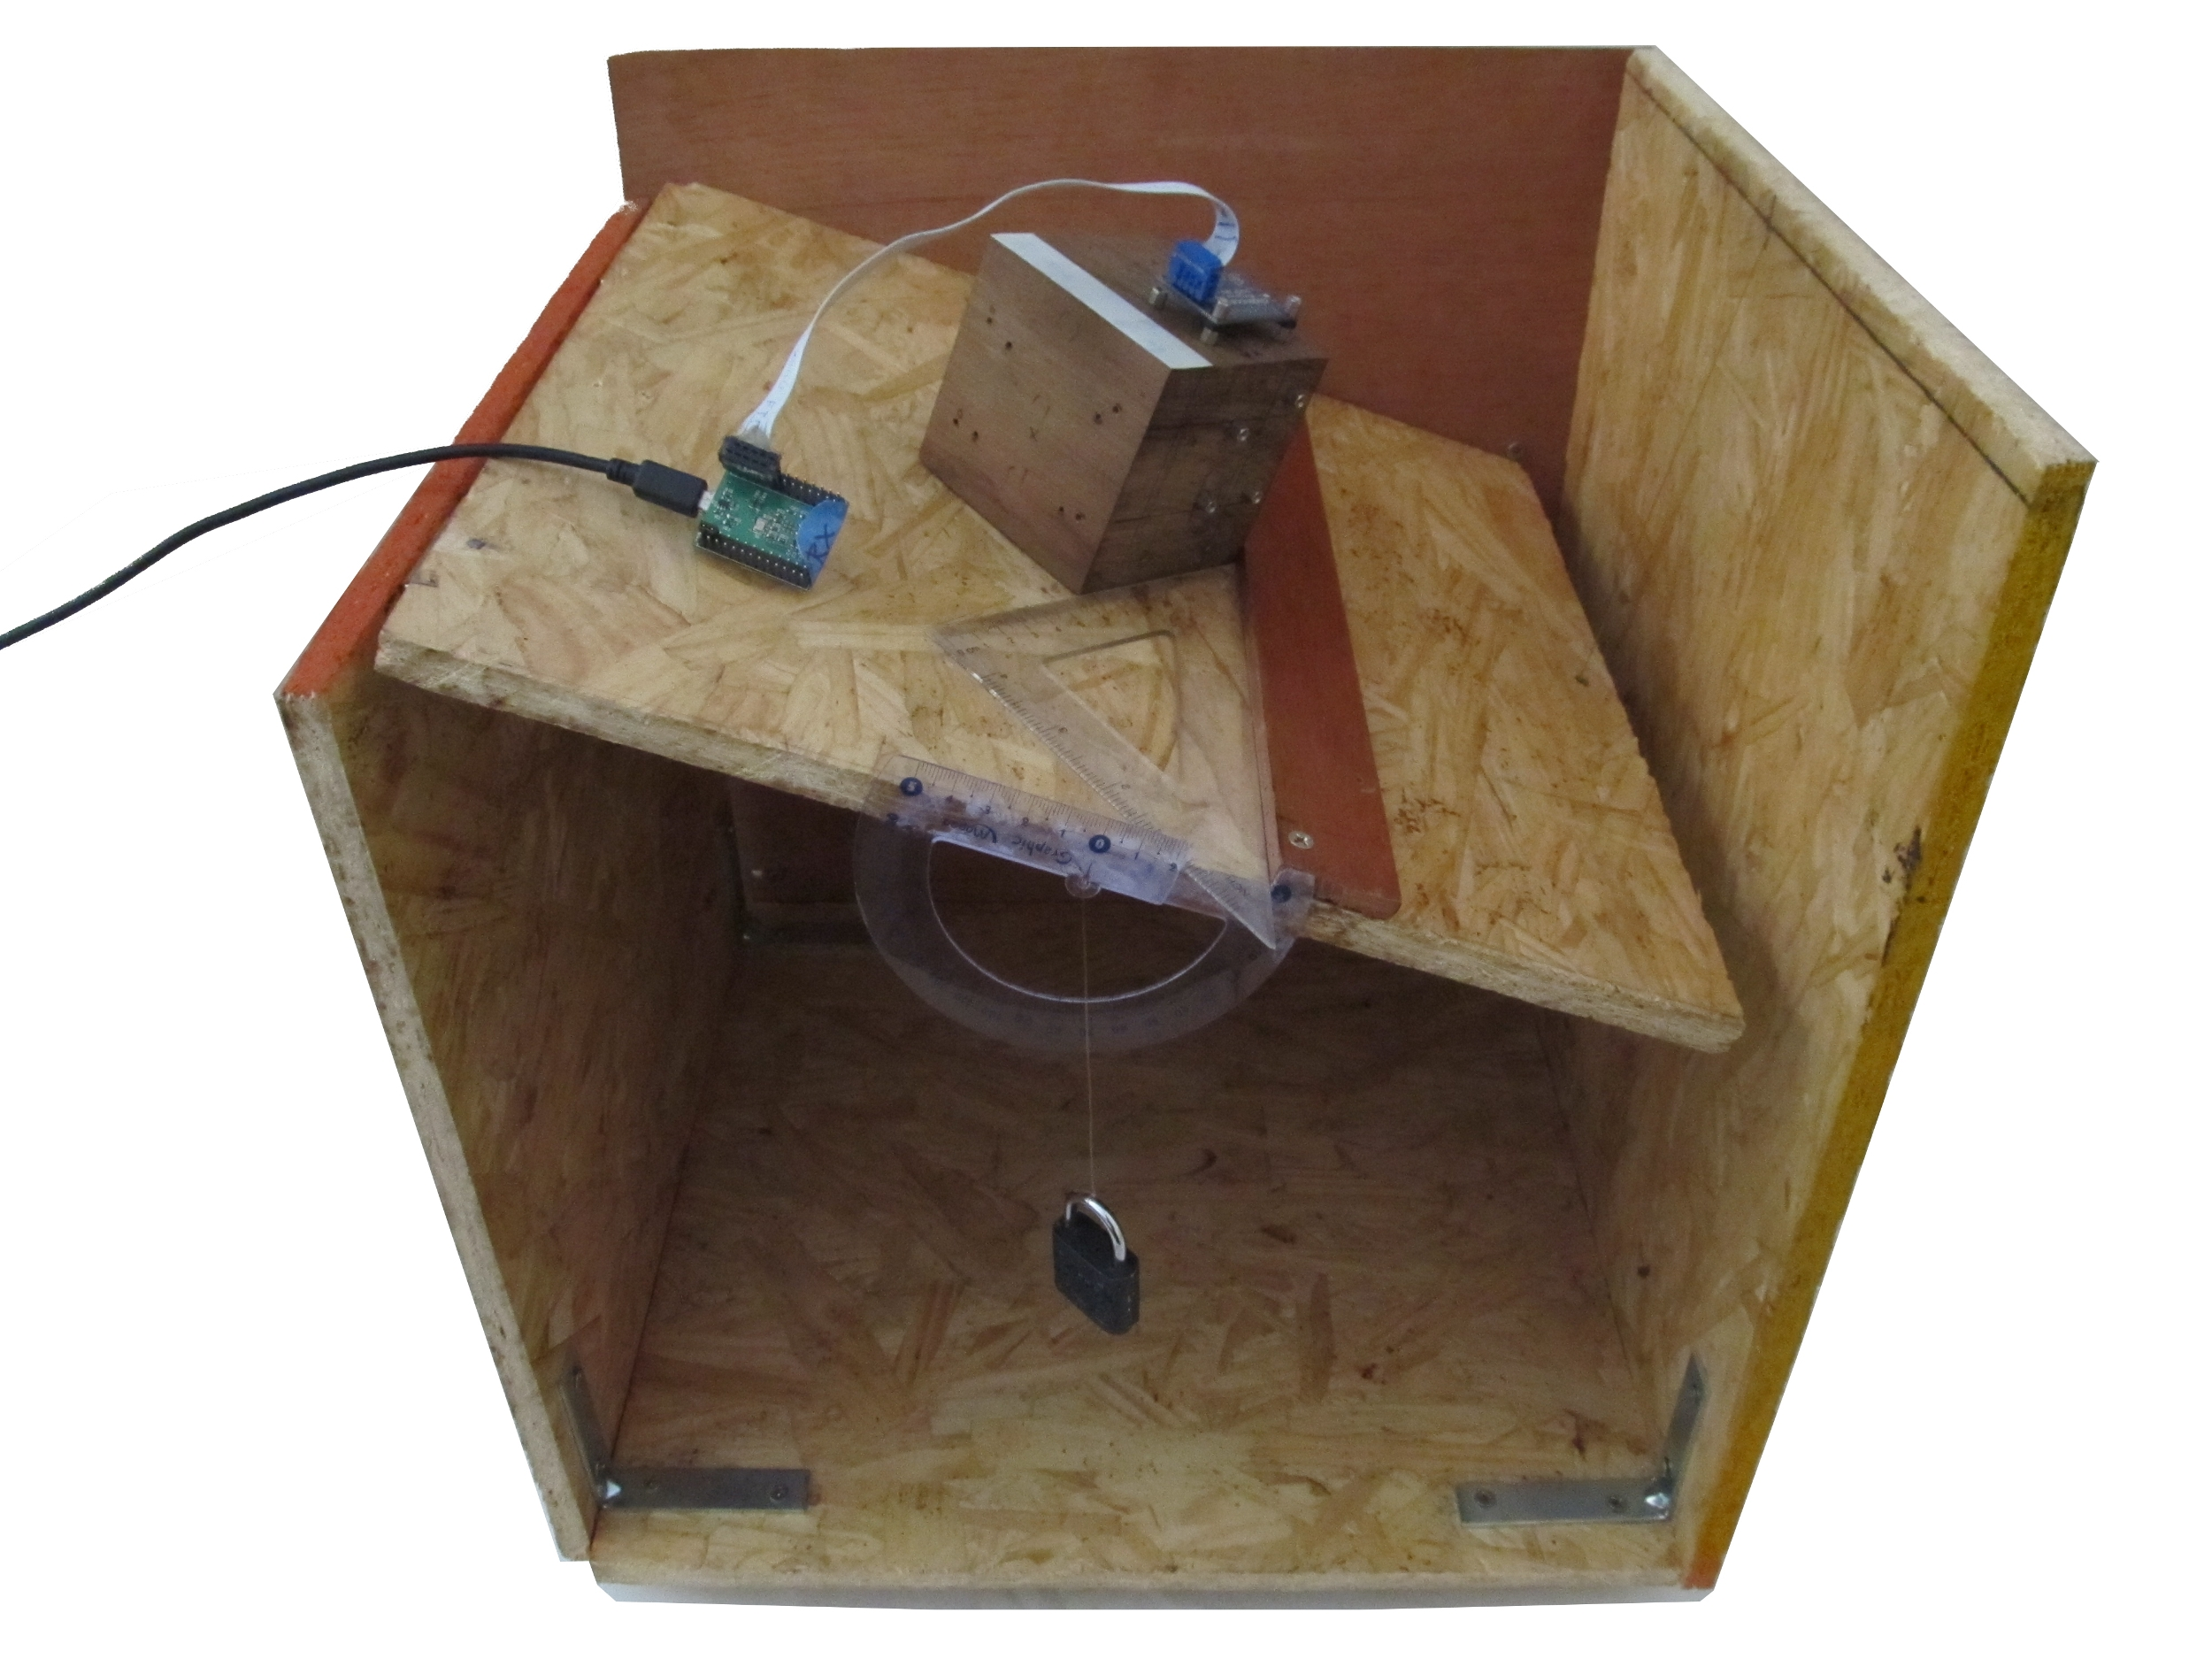
\includegraphics[width=.6\columnwidth]{./pics_paper/mesa.jpg}
	\caption{\textbf{Adjustable table}- Used for accelerometer calibration}
	\label{fig:mesa}
\end{figure}

\begin{figure}
	\centering
	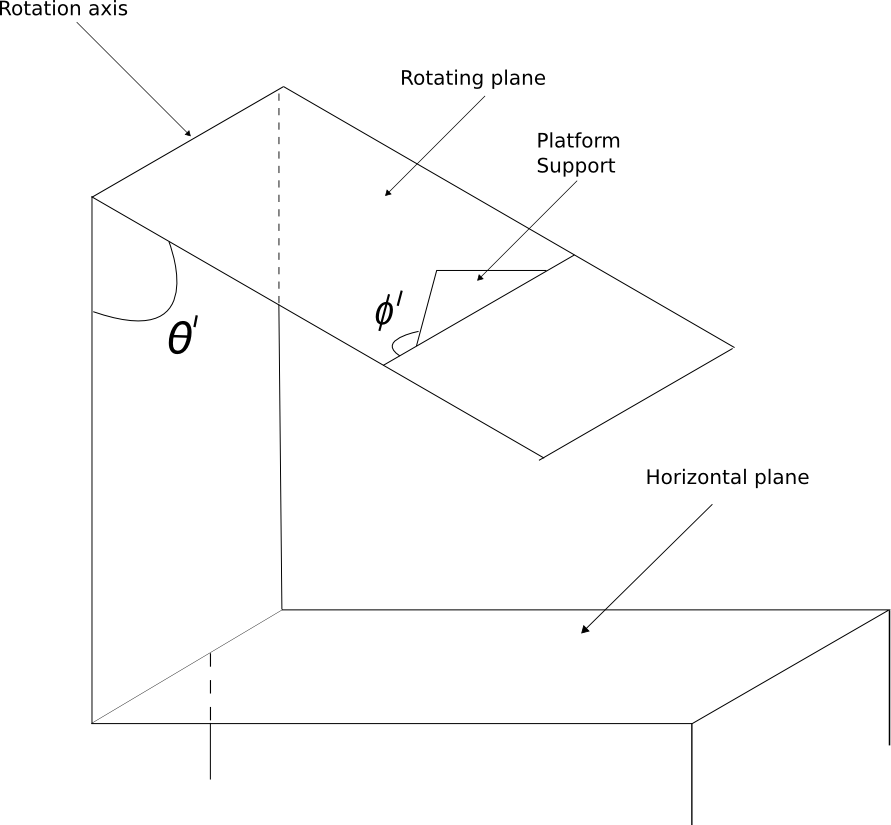
\includegraphics[width=.6\columnwidth]{./pics_paper/mesa_esquema.png}
	\caption{\textbf{Adjustable table}- Scheme}
	\label{fig:mesa_esquema}
\end{figure}

As it was stated in \refp{sec:modelo} the problem \refp{eq:calib_problem} may have more than one local minimum, thus it is needed to assure that the seed of the algorithm is ``near'' of the values of the parameters. The proposed way to generate such a seed is to use some information of the sensor's datasheet\cite{bib:acc_data}: 

\begin{itemize}
\item The typical sensitivity for each axis is $256 bits/g \approx 26.10 bits / m^{s-2}$.
\item The typical offset for each axis is $0 ms^{-2}$.
\item As the axis should be as orthogonal as possible is reasonable to think that the rotation angles $\alpha_{aij}$ are near zero. 
\end{itemize}

After this considerations the chosen seed is:
\begin{equation}
{\theta}_0 = [26.10, 26.10, 26.10, 0, 0, 0, 0, 0, 0, 0, 0, 0, 0, 0, 0]^T
\end{equation}
\subsubsection{Gyroscope}

The procedure used to calibrate the gyroscope was very similar to the accelerometer. The main idea is to obtain a constant and known angular speed vector and then change the orientation of the gyroscope to have different measures in each axis.\\

In this case the constant angular speed was provided with a turntable ($33 rev/min$). Its angular speed was measured just to be sure that it was working properly. Different orientations were obtained using the wooden cube mentioned in Section \refp{subsec:acc},to assure $90^\circ$ rotations and pairs of carpenter's squares to assure $30^\circ$, $45^\circ$ and $60^\circ$ rotations. In Figure \refp{fig:setup_gyro} is shown the setup that was mounted over the turntable.\\

As we did for the accelerometer, we are going to choose a seed based on the information in the device's datasheet \cite{bib:gyro_data}: 

\begin{itemize}
\item The typical sensitivity for each axis is $14,375 bits/(^\circ s^{-1})\approx 823.63 bits/(rad s^{-1})$.
\item The typical offset for each axis is $0 rad s^{-1}$.
\item As the axis should be as orthogonal as possible is reasonable to think that the rotation angles $\alpha_{\omega ij}$ are near zero. 
\end{itemize}

After this considerations the chose seed is:
\begin{equation}
{\theta}_0 = [823.63, 823.63, 823.63, 0, 0, 0, 0, 0, 0, 0, 0, 0, 0, 0, 0]^T
\end{equation}

\begin{figure}
	\centering
	\includegraphics[width=.6\columnwidth]{./pics_paper/escuadra.pdf}
	\caption{\textbf{Gyroscope setup - }Carpenter's squares were used to assure an exact orientation}
	\label{fig:setup_gyro}
\end{figure}


\subsection{Temperature adjust}
\label{sec:param_temp}

In this paper we also propose to realize a temperature adjustment. The sensors are exposed to the operating temperature of the system, and it is very common that this temperature is different from the calibration temperature. Sensors based in MEMS technology are sensitive to such variations. The variation of the measures is critical in some applications (see \cite{bib:uquad} for example). In INS two of the Euler angles are usually obtained from the accelerometer, therefore if the measures are not certain the stability of the system cannot be guaranteed.\\

It is extremely important to understand which of the parameters are affected based on the information of the sensors' datasheets (\cite{bib:acc_data} and \cite{bib:gyro_data}):

\begin{itemize}
\item Sensitivity variation of the accelerometer: $\pm 0.01 \%/^\circ C$
\item Offset variation of the accelerometer: $\pm 1.2mg/^\circ C \approx 0.012m s^{-1}$
\item Sensitivity variation of the gyroscope: No information is provided. 
\item Offset variation of the accelerometer: $\pm 40 ^\circ s^{-1} \approx 0.70 rad s^{-1}$
\end{itemize}

The conclusion of this sum up information is that the variations of the temperature do not produce main changes on the gains of the sensors, yet the offsets are modified. Thus, we are going to consider the following temperature adjust:

\begin{equation}
\mathbf{b}_s(T) = \mathbf{b}_{s0} + \boldsymbol{\alpha}_s (T-T_0)
\label{eq:temp}
\end{equation}

In equation \refp{eq:temp} $\mathbf{b}_{s0}$ is the offset vector obtained in the static calibration, $T_0$ is the ambiance temperature in the calibration, $T$ is the working temperature of the system and $\boldsymbol{\alpha}_s$ is the parameter that we need to know to complete the process.\\ 

The procedure to achieve this adjust was take several samples of acceleration (or angular speed) in a fixed position ($z$ axis pointing ``up'' without any rotation), while the sensor was heat up with a hair dryer. The criterion chose was that $\boldsymbol{\alpha}_s$ must minimize the sum of the squares of the norms of the difference between the true acceleration (or angular speed) and the measured acceleration (or angular speed). Mathematically this means:

\begin{equation}
\min_{\boldsymbol{\alpha}_s} = \sum_{k=1}^N ||\mathbf{s}_i^p - \mathbf{T}_{s0}^p(\mathbf{K_{s0}})^{-1}(\tilde{\mathbf{s}}_i^s-\mathbf{b}_s(T))||^2 
\label{eq:calib_temp}
\end{equation}

In equation \refp{eq:calib_temp}, $N$ is the number of samples took, $\mathbf{T}_{s0}^p$, $\mathbf{K_{s0}}$ are the matrix obtained in the static parameter calibration (ambiance temperature) and $\mathbf{b}_s(T)$ is the vector defined in \refp{eq:temp}. This last vector includes the variable that we want to estimate.\\

\section{Results and analysis}
\subsection{Static parameters}
In this section, the parameters that solve problem \ref{eq:calib_problem} are presented for both accelerometer and gyroscope. In addition, the statistic over the test set is studied and analyzed. \\

\subsubsection{Accelerometer}
The parameter vector found in this case is:
\begin{eqnarray}
\boldsymbol{\theta}_a &=& [26.70, 27.26, 26.02, 16.05, -1.79, -47.99,\\ \nonumber
&& 3,78\times 10^{-4}, 1.40\times 10^{-3}, 1.63 \times 10^{-2},  4.62 \times 10^{-3},\\ \nonumber
&& -2.30\times 10^{-3}, -6.81 \times 10^{-3}]^T \nonumber
\end{eqnarray}

It is interesting to compare the values obtained with the theoretical values of each parameter. As we can see, comparing the vector obtained with the seed, the values of the gains and the rotations are similar to what is declared in the datasheets. However the offset values obtained differ considerably from the information of the datasheet (see \cite{bib:acc_data}), where is declared that the 0g output deviation from ideal is $\pm 35 mg$ for axes $x$ and $y$ and $\pm 40mg$ for axis $z$. This means that the offsets should be less than $11$ bits, therefore a difference between the results obtained in the calibration and what is stated in the datasheet of the sensor exists.\\

The mean error, and the standard deviation founded with the calibration method proposed in the test set are:

\begin{equation}
\mu_a = -0.03ms^{-2}, \; \sigma_a = 0.06ms^{-2}
\end{equation}

The mean error obtained correspond to less that a bit of error and the standard deviation to a bit and a half. Therefore we can conlude that a very good calibration has been achived for the static parameters of the accelerometer.\\

At first appearance it does not seems right that the accuracy of the results is comparable with the instrument resolution. However, this fact can be explain because the effect of electrical noise. Let's suppose that the true acceleration correspond to $128.2$ bits. If the accelerometer was ideal a constant lecture of $128$ bits would be obtained. However, due to the electrical noise the value of the measure obtained varies typically one or two bits (see Figure \refp{fig:noise}). Those variations are not uniform, on the contrary, they depend on the true value of the acceleration. In the considered case the value $128$ will be more common that the value $129$, yet if the true acceleration correspond to $128.74$ bits, the opposite would happen. To sum up, the electrical noise behaves in a way that depends on the true value of the acceleration. Thus, taking an average of almost $20000$ samples per measure ($20$ seconds of data), the obtained value is more accurate than the resolution of the instrument is obtained. \\


\subsubsection{Gyroscope}
For the gyroscope the vector of parameters obtained is the following:

\begin{eqnarray}
\boldsymbol{\theta}_\omega &=& [792.44,\, 808.61, \, 799.44, \, -33.52, \, -31.41, \\ \nonumber
& & -1.07, \, 0.02, \, 0.06, \, -1.32 \times 10^{-3}, \, 2.59\times 10^{2}, \, \\ \nonumber
& & -3.25 \times 10^{-2}, \, 6.07\times 10^{-1}]^T \nonumber
\end{eqnarray}

As we can see the gains are very similar to the ones that are declared on the datasheets. The maximum relative error obtained is:

\begin{equation}
\varepsilon_{\omega gain} = \frac{|823.63 - 792.44|}{823.63} = 3.8 \%
\end{equation}

On the other hand, the typical offset error is $\pm 40 ^\circ s^{-1}$, this correspond to an error of $\pm 574 bits$. All the offsets estimated are smaller than this value, representing in the worst case only the $5.8 \%$ than the maximum declared in the datasheets. \\

Last but not least, the results over the test set are the following:

\begin{equation}
\mu_\omega = 6.67 \times 10^{-3} rad/s\, \sigma_\omega = 7.4 \times 10^{-3} rad/s
\end{equation}

The mean and the standard deviation obtained both correspond to approximately $6$ bits errors.

As we can see the error obtained, in terms of bits, is bigger for the gyroscope than for the accelerometer. The main reason for this to happen is that in this case we are working with a scale that is not optimal, yet the only one available, for the speed of interest. The maximal angular speed measured ($198 ^{\circ} /s$ ) is approximately a tenth of the scale of the gyroscope ($2000^{\circ} /s$) while for the accelerometer the maximal acceleration measured ($g$) is the half of the scale used ($2 g$). 

\subsection{Temperature adjust}

To evaluate the behavior of the measurement of the accelerometer and compensate the error caused by temperature, the experiment described in Section \refp{sec:param_temp} is carried out. It can be divided in two separate parts, the first is heating up the sensor using a hair dryer up to $48^oC$ and the second part is letting the sensor cool down to normal operating temperature. The two separated parts of the experiment are shown in Figures \refp{fig:resultado_temp} and \refp{fig:bajada}.

\begin{figure}
	\centering
	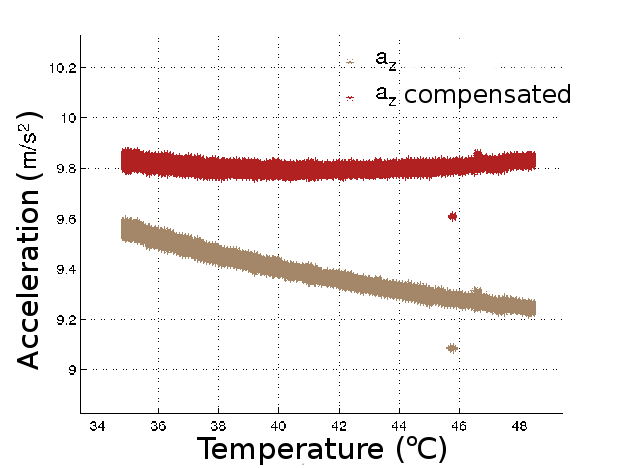
\includegraphics[width=.8\columnwidth]{./pics_paper/resultado_temp.png}
	\caption{\textbf{Gyroscope setup - }Accelerometer measurement in z-axis vs. temperature while heating up the sensor.}
	\label{fig:resultado_temp}
\end{figure}
\begin{figure}
	\centering
	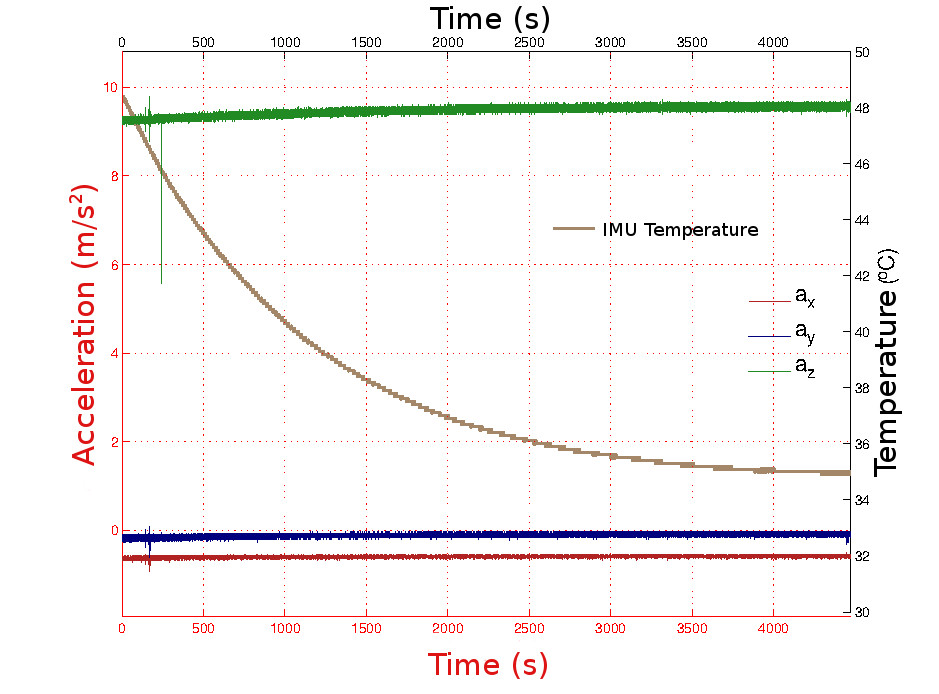
\includegraphics[width=.8\columnwidth]{./pics_paper/bajada.png}
	\caption{\textbf{Gyroscope setup - }Accelerometer measurements and temperature (T) vs. time while T varying from $35^oC$ to $48^oC$.}
	\label{fig:bajada}
\end{figure}

\balance
In Figure \refp{fig:resultado_temp} is shown the behavior of the calibrated measurement of the accelerometer in z-axis while the sensor is heated up, both with and without temperature compensation. It is clearly shown that the compensated temperature is much more reliable than the other one, that is varying a 3\% of the highest value. Otherwise, in Figure \refp{fig:bajada} the second part of the experiment is shown, letting the sensor cool down up to normal operating temperature. Two different magnitudes are shown at the same time: the three accelerations and the temperature, thus two axes are needed to be shown: on left side the acceleration in $ms^{-2}$, and on right side the temperature in $^oC$.\\
In Figure \refp{fig:resultado_temp} can be observed that at about the end of the experiment the sensor output is $9.25ms^{-2}$ instead of $9.81ms^{-2}$, which means an error of $0.56ms^{-2}$. Such an error in acceleration measurements can cause several errors in applications where the operating temperature can differ from the calibration temperature, thus, is vital that temperature compensation is performed.


\section{Conclusion}

% use section* for acknowledgement

% trigger a \newpage just before the given reference
% number - used to balance the columns on the last page
% adjust value as needed - may need to be readjusted if
% the document is modified later
%\IEEEtriggeratref{8}
% The "triggered" command can be changed if desired:
%\IEEEtriggercmd{\enlargethispage{-5in}}

% references section

% can use a bibliography generated by BibTeX as a .bbl file
% BibTeX documentation can be easily obtained at:
% http://www.ctan.org/tex-archive/biblio/bibtex/contrib/doc/
% The IEEEtran BibTeX style support page is at:
% http://www.michaelshell.org/tex/ieeetran/bibtex/
%\bibliographystyle{IEEEtran}
% argument is your BibTeX string definitions and bibliography database(s)
%\bibliography{IEEEabrv,../bib/paper}
%
% <OR> manually copy in the resultant .bbl file
% set second argument of \begin to the number of references
% (used to reserve space for the reference number labels box)
\bibliographystyle{ieeetr} 
\bibliography{../biblio}
% \begin{thebibliography}{1}

% \bibitem{IEEEhowto:kopka}
% H.~Kopka and P.~W. Daly, \emph{A Guide to \LaTeX}, 3rd~ed.\hskip 1em plus
%   0.5em minus 0.4em\relax Harlow, England: Addison-Wesley, 1999.
% \end{thebibliography}

% that's all folks
\end{document}


